\documentclass{../notatki}

\title{Elektryczność i Magnetyzm}

\usetikzlibrary{calc}

\begin{document}

\tableofcontents

\section{Literatura}

\begin{itemize}
  \item E. M. Purcell, D. J. Morin "Electricity and Magnetism"
  \item R. Shankar "Fundamentals of Physics II"
  \item OpenStax
    \href{https://assets.openstax.org/oscms-prodcms/media/documents/College_Physics_2e-WEB_7Zesafu.pdf#%5B%7B%22num%22%3A2876%2C%22gen%22%3A0%7D%2C%7B%22name%22%3A%22XYZ%22%7D%2C0%2C734%2C0%5D}{"College
    Physics"}
\end{itemize}

\section{Cząstki}

Elektryczność jest zjawiskiem, wynikającym z oddziaływań pomiędzy nukleonami.
Wyróżniamy trzy nukleony: proton, neutron i elektron. Proton ma ładunek dodatni,
neutron jest obojętny, a elektron ma ładunek ujemny. Proton i neutron znajdują
się w jądrze atomowym, które choć zmienne w wyniku reakcji jądrowych, jest
stabilne w warunkach normalnych. Elektrony z kolei krążą wokół jądra w tzw.
chmurze elektronowej. W wyniku oddziaływań pomiędzy innymi nukleonami elektrony
mogą być oderwane od atomu, tworząc jon dodatni lub ujemny. Tymczasowy brak
równowagi, gradient ładunku, w materiale złożonym z kilku cząstek
jest przyczyną zjawisk elektrycznych.

\section{Przewodniki}

Wyróżniamy grupę materiałów, które w wyniku ich struktury atomowej pozwalają na
swobodny transfer elektronów i powstawanie gradientu ładunku. Są to przewodniki.
Metale w wyniku istnienia specjalnych wiązań chemicznych są dobrymi
przewodnikami.
Podobnie roztwory elektrolityczne, w których jony mogą swobodnie
przemieszczać się
w roztworze. W przeciwieństwie do przewodników, izolatory nie
pozwalają na swobodny
transfer elektronów. W wyniku tego nie powstaje gradient ładunku.

\section{Ładunek}

Ładunek danej dyskretnej cząsteczki jest wielkością skalarną określoną wzorem:
$$
q = n \cdot e
$$
gdzie $e$ to ładunek elementarny($1.6 \cdot 10^{-19} C$), a $n$ to liczba
cząsteczek.
\textbf{Suma ładunków w układzie izolowanym jest stała.}

\section{Elektryzowanie}

W wyniku różnych oddziaływań pomiędzy ciałami, mogą one nabrać
ładunku. Wyróżniamy
kilka metod elektryzowania ciał. W każdej z nich powstaje gradient ładunku.

\subsection{Elektryzowanie przez tarcie}

W wyniku tarcia między ciałami, elektrony mogą być przenoszone z
jednego ciała na
drugie. W wyniku tego jedno ciało nabiera ładunku dodatniego, a drugie ujemnego.

\subsection{Elektryzowanie przez dotyk}

W momencie, w którym dotkniemy dwa ciała o różnym ładunku
przewodnikiem, elektrony
przenoszą się z ciała o większym ładunku do ciała o mniejszym
ładunku. W wyniku tego
oba ciała nabierają ładunku o wartości pośredniej.

\subsection{Elektryzowanie przez indukcję}

W wyniku zbliżenia ciała o ładunku do ciała obojętnego, ładunek
w ciele obojętnym jest przemieszczany w wyniku oddziaływań pomiędzy
ładunkami. W wyniku tego ciało obojętne nabiera ładunku. W materiałach
przewodzących ładunek jest przemieszczany swobodnie, w izolatorach gradient
powstaje w wyniku polaryzacji cząsteczek.

\section{Prawo Coloumba}

Ciała naelektryzowane oddziałują na siebie zgodnie z prawem Coloumba:
$$
\vec{F} = k \cdot \frac{q_1 \cdot q_2}{r^2} \cdot \vec{r}
$$
gdzie $k$ to stała elektrostatyczna($\frac{1}{4\pi\epsilon_0}$,
$\epsilon_0\approx8.854\cdot10^{-12}\frac{F}{m}$).

\subsection{Zasada superpozycji}

Siła wypadkowa działająca na ciało naelektryzowane jest sumą sił
działających na to ciało ze strony innych ciał.
$$
\vec{F_w} = k \cdot \sum_{j=1}^{n} \frac{q_1 \cdot q_j}{r^2} \cdot \vec{r}
$$

\subsection{Przykład}

\begin{figure}[h]
  \centering
  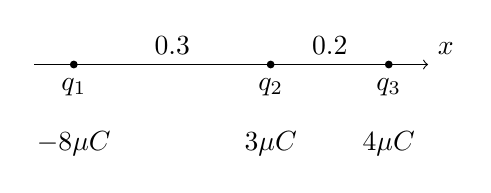
\begin{tikzpicture}
    \draw[->] (0,0) -- (5,0) node[above right] {$x$};
    \node[circle,fill,inner sep=1pt,label=below:$q_1$] (q1) at (0.5,0) {};
    \node[circle,fill,inner sep=1pt,label=below:$q_2$] (q2) at (3,0) {};
    \node[circle,fill,inner sep=1pt,label=below:$q_3$] (q3) at (4.5,0) {};
    \draw[] (q1) -- (q2) node[midway,above] {$0.3$};
    \draw[] (q2) -- (q3) node[midway,above] {$0.2$};
    \node[below of=q1] {$-8\mu C$};
    \node[below of=q2] {$3\mu C$};
    \node[below of=q3] {$4\mu C$};
  \end{tikzpicture}
\end{figure}
$$
\vec{F_{31}} = k \cdot \frac{q_1 \cdot q_3}{r^2} = k \cdot \frac{-8\cdot
4}{0.5^2} = -1.2 N
$$
$$
\vec{F_{32}} = k \cdot \frac{q_1 \cdot q_2}{r^2} = k \cdot \frac{3\cdot
4}{0.2^2} = 2.7 N
$$

\section{Pole elektryczne}

Pole elektryczne jest polem wektorowym, które opisuje siłę działającą na
naelektryzowane ciało. Pole elektryczne jest zdefiniowane jako:
$$
\vec{E} = \frac{\vec{F}}{q}
$$
gdzie $\vec{F}$ to siła działająca na ciało o ładunku $q$.

\subsection{Linia pola elektrycznego}

Do obrazowego przedstawienia pola elektrycznego używamy linii pola
elektrycznego. Linie pola elektrycznego to linie które w każdym punkcie są
styczne do wektora siły pola elektrycznego. Są one przedstawiane jako dyskretne
linie, lecz w rzeczywistości pole elektryczne jest ciągłe.

\subsection{Natężenie pola elektrycznego}

Natężenie pola elektrycznego to wielkość wektorowa, która opisuje siłę
działającą na jednostkowy ładunek w danym punkcie pola elektrycznego.
$$
E = k \cdot \frac{|q|}{r^2}
$$
Obowiązuje zasada superpozycji.

\section{Dipol elektryczny}

Dipol elektryczny to układ dwóch ładunków o równych wartościach, lecz
przeciwnych znakach. W wyniku tego układu powstaje pole elektryczne, które
jest zależne od odległości między ładunkami. W wyniku tego dipol elektryczny
jest zawsze zorientowany w kierunku od ładunku dodatniego do ujemnego.

\begin{figure}[h]
  \centering
  \begin{tikzpicture}
    \node[circle,fill,inner sep=1pt,label=below:$q_+$] (q1) at (0,0) {};
    \node[circle,fill,inner sep=1pt,label=below:$q_-$] (q2) at (2,0) {};
    \draw[-] (q1) -- (q2) node[midway,above] {$d$};
  \end{tikzpicture}
\end{figure}

\end{document}